\documentclass{article}
\usepackage{nips15submit_e, times}
\usepackage{amsmath}
\usepackage{amsfonts}
\usepackage{algorithm}
\usepackage{algorithmicx}
\usepackage{algpseudocode}
\usepackage{booktabs}
\usepackage{graphicx}
\usepackage{subfigure}
\usepackage{placeins}
\usepackage{enumerate}
\usepackage{diagbox}
\usepackage{tocbibind}

\title{Face Aging using Generative Adversarial Network}
\date{March 2019}
\begin{document}
\maketitle
\begin{abstract}
Recent studies have shown remarkable success in image-to-image translation for two domains. We especially focused on using StarGAN and a proposed novel model named AE-cDCGAN. By exploring cDCGAN, we observed that it can generate elder and young faces with random noise vector. By plugging an encoder component to the generator and another MSE term to generator's loss function. Finally, compared with StarGAN, AE-cDCGAN can complete face aging task but look less clear. In otder to generate most reasonable face, we tuned $\alpha$ parameter as 10. For the training time, StarGAN takes 37 mins but AE-cDCGAN takes 26 mins for one epoch, which means our proposed models is a lightweight framework.
\end{abstract}

\section{Introduction}
In recent years, generative adversarial network achieve well-performed result. It can be applied into many fields. The initial focus for GAN is to generate data from a noise vector, such as image, music and etc. However, the scope of it is far larger than to be a generative model. For example, it can help a image to complete a domain transfer. Or it also can helps a robot to learn faster in reinforcement learning. 
\par In this final report, our group plans to utilize conditional version of GAN to enable a face to be aging. The state of art is Star-GAN, which can be applied to complete image domain transformation. In this project, we firstly set Star-GAN\cite{DBLP:journals/corr/abs-1711-09020} to complete face aging. Besides, we proposed a modified version of cDCGAN to accept an original image and transform it into elder faces. To be specific, we plugged an encoder component into the generator to accept original image and plugged another mean square error term into loss function of generator. Intuitively, what we expect with this model is to accept an image and preserve the identity.

\section{Related Works}
The deep generative networks have exhibited a remarkable capability in image generation and have also been investigated for age progression. These approaches render faces with more appealing aging effects and less ghosting artifacts compared to the previous conventional solutions. Specifically, these approaches truly aims to complete image domain translation instead of focusing on face aging. However, the essence of face aging should both preserve the identity and modify the age related characteristics simultaneously. In addition, some of the works works fine for more concrete age stage. For example, Yang\cite{Yang2017Learning} proposed a model to generate faces under different ages instead of just young and elder. 

\section{Methodology}
\subsection{Dataset}
CelebFaces Attributes Dataset (CelebA) \cite{liu2015faceattributes} is a large scale face attributes dataset with more than 200k celebrity images, each with 40 attributes. CelebA has large diversities, large quantities and rich annotations including 10,177 number of identities, 202,599 number of face images and 5 landmark locations, 40 binary attributes per image.

For the face aging task, we specifically focus on age attribute which will be the additional input to the generative adversarial network so that we can guide the network to generate images of the same identity in different ages. Due to the time limitation, we will not train the CDC-GAN and StarGAN on the whole CelebA dataset instead using a portion of it.

Figure \ref{data sample} shows some sample images from CelebA dataset. We will crop the initial 218$\times$178 size images to 178$\times$178 then resize images as 128$\times$128.

\begin{figure}[H]
\begin{center}
  \centering
  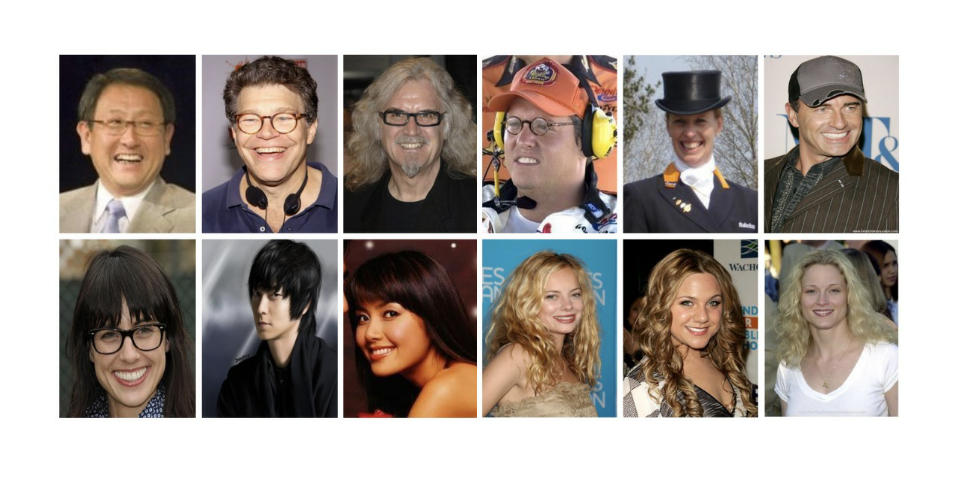
\includegraphics[width=5in]{image/data_sample.png}
\end{center}
\caption{Sample images from CelebA dataset.}
\label{data sample}
\end{figure}

\subsection{cDCGAN}
In the original work, GAN is able to gradually utilized to generate clear images. However, both vanilla GAN and DCGAN are not directed by the user whereas it generates the result randomly. In order to control the content generated, the model should be feed with some additional information. In this project, we are attempting to generate face images of a specific age based on the celebA training data set. Mirza et al.\cite{2014arXiv1411.1784M} introduced a novel way to train generative model known as conditional adversarial networks. Generative adversarial networks can be extended to a conditional model by conditioning both the generator and discriminator on some additional input, for example age in this task. Besides, by designing the generator and discriminator to be deep convolutional architecture extends the cGAN to conditional deep convolutional generative adversarial networks (cDCGAN). In our project, we designed the architecture as the following. Figure \ref{cdcgan_g} and Figure \ref{cdcgan_d} respectively show the architecture of generator and discriminator.

\begin{figure}[H]
\begin{center}
  \centering
  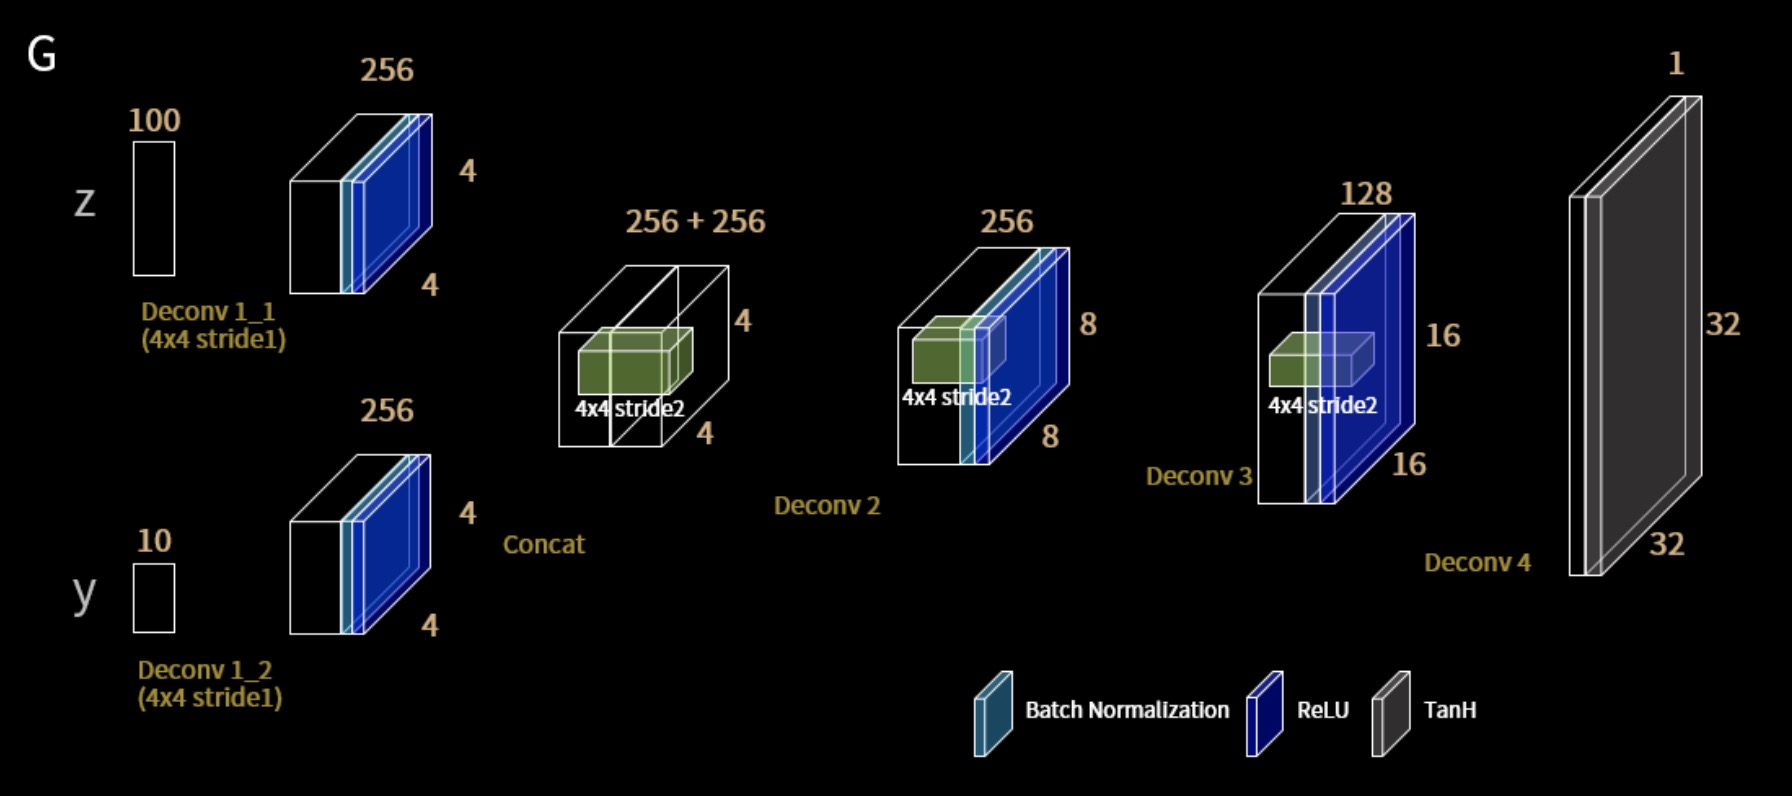
\includegraphics[scale=0.2]{image/cdcgan_g.png}
\end{center}
\caption{Generator of cDCGAN}
\label{cdcgan_g}
\end{figure}

\begin{figure}[H]
\begin{center}
  \centering
  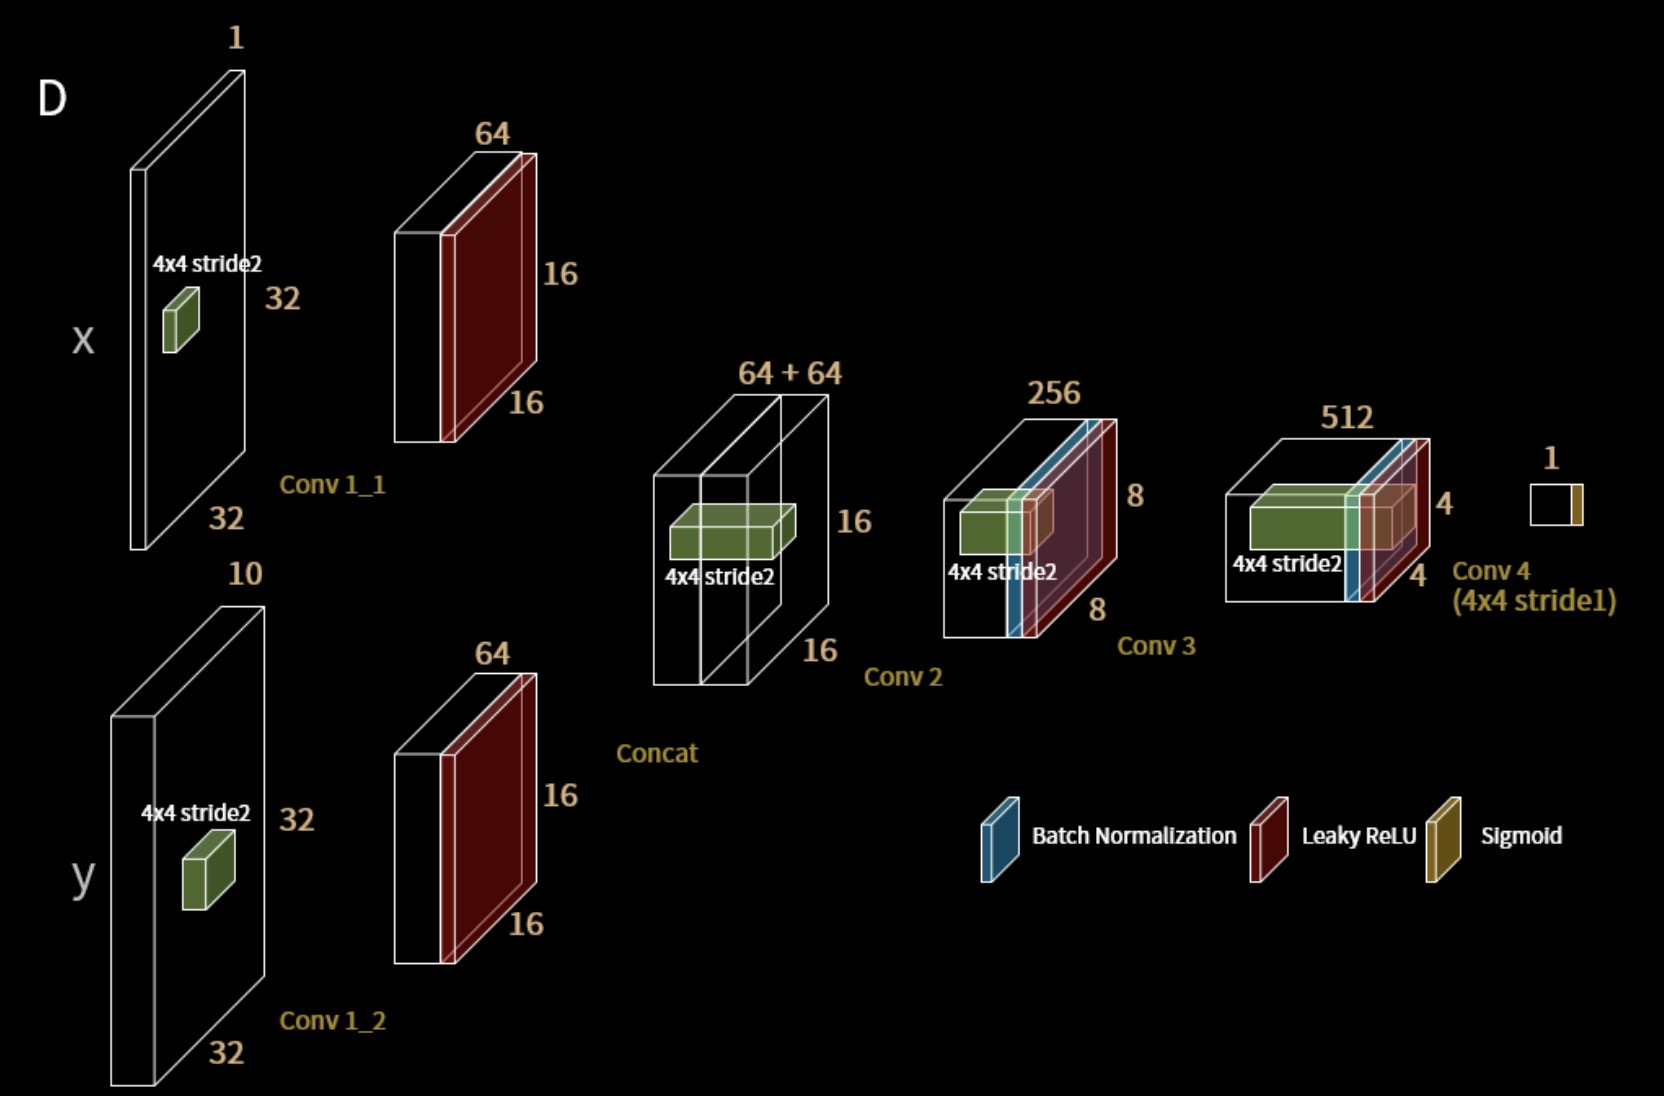
\includegraphics[width=5in]{image/cdcgan_d.png}
\end{center}
\caption{Discriminator of cDCGAN}
\label{cdcgan_d}
\end{figure}
The objective function for GAN model is a minmax function described in Equation (\ref{los function}). We expect both D(x) converging to zero and D(G(z)) converging to one.
\begin{equation}
\begin{split}
\text{minmax}(D,G)=E_{x~P(data)}[log(D(x))]+E_{z~p(z)}[log(1-D(G(z)))]
\end{split}
\label{los function}
\end{equation}
However, the input of cDCGAN is a random noise vector and the output is both the elder faces and young faces in this situation, which is different from what we plans to complete in this project. Therefore, we proposed a modified version of cDCGAN, named AE-cDCGAN. The architecture of AE-cDCGAN shows in Figure \ref{AE-cDCGAN}. The motivation of this architecture is to utilize an encoder to encode an input image. Besides, one of the problem for this proposed model is identity preservation, which means the generated face should be the same identity as the original person. In order to achieve this goal, another auto encoder loss function term was plugged into the Generator loss function like Equation \ref{equation: AE_loss}.
\begin{figure}[H]
\begin{center}
  \centering
  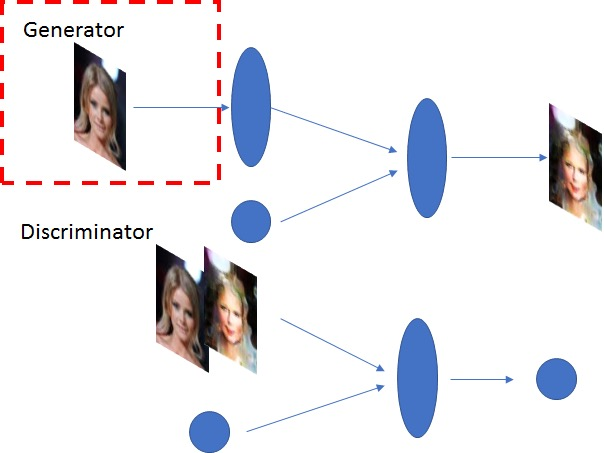
\includegraphics[scale=0.5]{image/cdcgan_structure.jpg}
\end{center}
\caption{Architecture of AE-cDCGAN}
\label{AE-cDCGAN}
\end{figure}

\begin{equation}
\begin{split}
L &= L_G + L_D\\
L_D &= BCELoss(D(x_T,y),1) + BCELoss(D(G(x,y),y),0)\\
L_G &= BCELoss(D(G(x,y),y),1) + \alpha MSE(x,G(x,y))\\
\end{split}
\label{equation: AE_loss}
\end{equation}

\subsection{StarGAN}
Y. Choi et al. \cite{DBLP:journals/corr/abs-1711-09020} introduce a novel and scalable approach that can perform image-to-image translations for multiple domains using only a single model.

Figure \ref{stargan} shows the overall structure of StarGAN which consists of two modules, a discriminator $D$ and a generator $G$. Basically, \textbf{(a)} $D$ learns to distinguish the real images from fake one and classify the real images to its domain. \textbf{(b)} Both target domain and input images are fed into $G$ to generate the fake image. \textbf{(c)} $G$ tries to reconstruct the original images by using the fake image and the original domain of real image. textbf{(d)} $G$ tries to generate images that are indistinguishable from the real images and the domain classified by $D$.

\begin{figure}[H]
\begin{center}
  \centering
  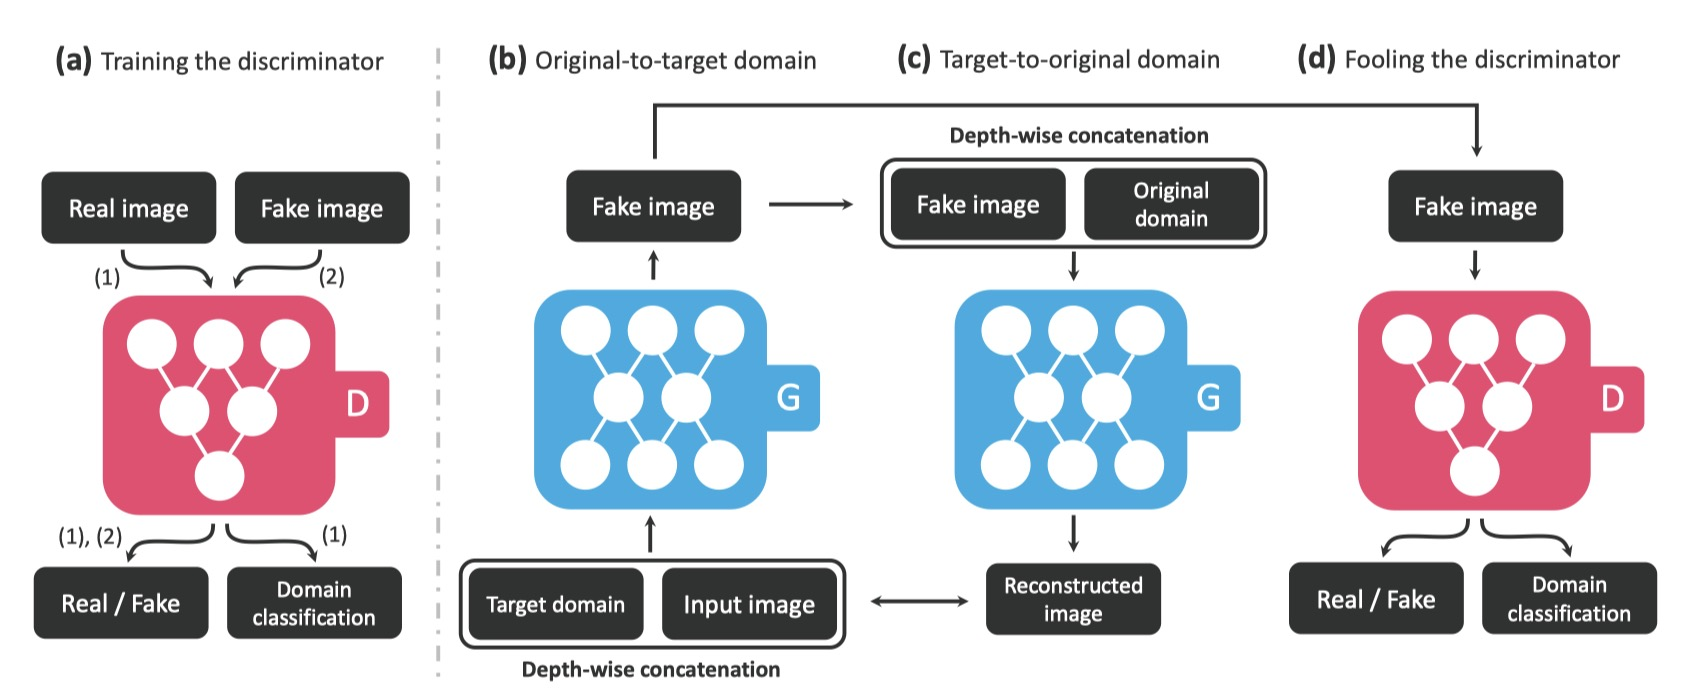
\includegraphics[width=5in]{image/stargan.png}
\end{center}
\caption{Overview of StarGAN.}
\label{stargan}
\end{figure}

\section{Experiments and Results}
In this section, we will first show the result of cDCGAN and Star-GAN respectively. Further, we will design some experiments to compare the performance of the two models.
\subsection{Result of cDCGAN}
In the model, we confronted several issues during training the model. First all, in celebA dataset, the fraction of elder faces and young faces are significantly imbalanced, which leads to the generator hard to generate clear faces. To be specific, there are 40k elder faces and 150k younger faces in the celebA dataset. In this situation, the generated images looks fuzzy like Figure \ref{figure: fuzzy}.
\begin{figure}[H]
\begin{center}
  \centering
  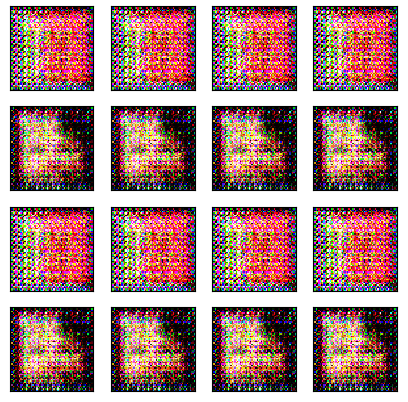
\includegraphics[scale=0.6]{image/fuzzy.png}
\end{center}
\caption{Imbalanced elder faces and young faces lead the generator hard to train.}
\label{figure: fuzzy}
\end{figure}
In order to enable the training set to be balanced and simultaneously utilized as more original as possible to generate clear images. Therefore, we solved this issue with the following procedure showing in Algorithm \ref{alg:train}.
\begin{algorithm}
        \caption{Training Process}
        \label{alg:train}
        \begin{algorithmic}[1]
             \State randomly choose 40k young faces and combine it with 40k elder faces as one data loader
             \State Similarly, we utilized the 40k elder faces again and choose another 40k young faces. Repeat the same procedure again. And finally, we obtained three data loaders which contain 40k elder faces and 40k older faces.
             \State During the training, those three data loaders are iterated once in one epoch
        \end{algorithmic}
\end{algorithm}
Figure \ref{cdcgan_loss} shows the loss change of cDCGAN. From the figure, we can find that the loss of discriminator doesn't change much compared with the generator. At the $epoch=1$, there's a large drop of the generator's loss, and so the loss of discriminator increases a little bit, which can be explained by the mutual inhibition relationship between them. When the model becomes converge, the loss of both generator and discriminator will not change.
\begin{figure}[H]
\begin{center}
  \centering
  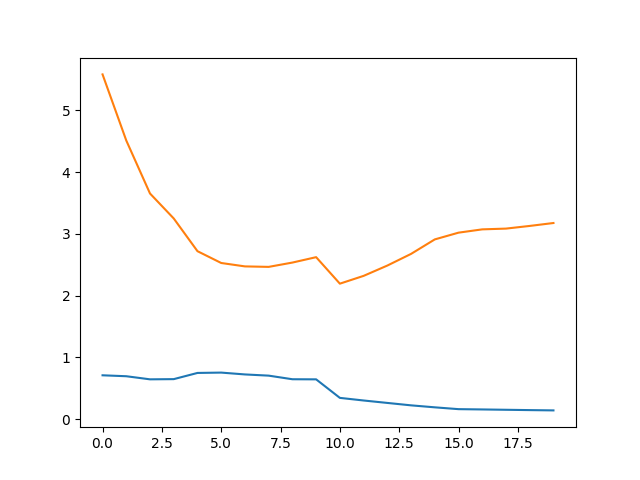
\includegraphics[width=3.3in]{image/cgan_loss.png}
\end{center}
\caption{Loss change of cDCGAN over 20 epochs. The orange line shows the loss of generator. The blue line shows the loss of discriminator.}
\label{cdcgan_loss}
\end{figure}


\subsubsection{Variation across the epoch}
Figure \ref{epoch_variation} shows the generated young faces and elder faces under different epoch. All of the images in this figure are generated by a fixed random noise. Therefore, all of the faces in the figure are similar. From left to right, the face gradually becomes clear and then becomes blurred, which matches the generator loss curve in Figure \ref{cdcgan_loss}.

\begin{figure}[H]
\begin{center}
  \centering
  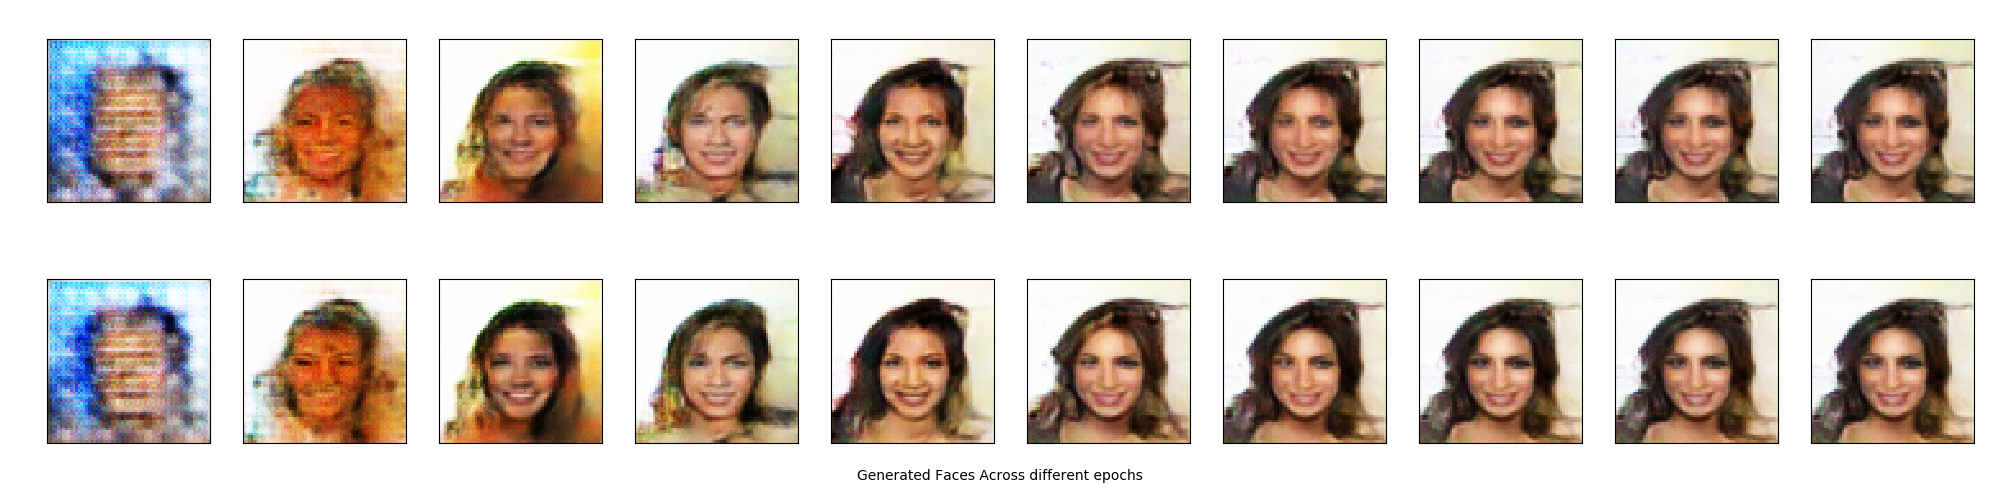
\includegraphics[width=5in]{image/epoch_variation.png}
\end{center}
\caption{Generated faces under different epochs. The first row represents the result of elder faces under different epochs. The second row represents the generated young faces under different epochs.}
\label{epoch_variation}
\end{figure}


\subsubsection{Generated faces across different identities}
Figure \ref{figure: diff_identity} shows the generated faces across different fixed noises which stands for different identities. The first row represents the elder faces and the second stands for the young faces.
\begin{figure}[H]
\begin{center}
  \centering
  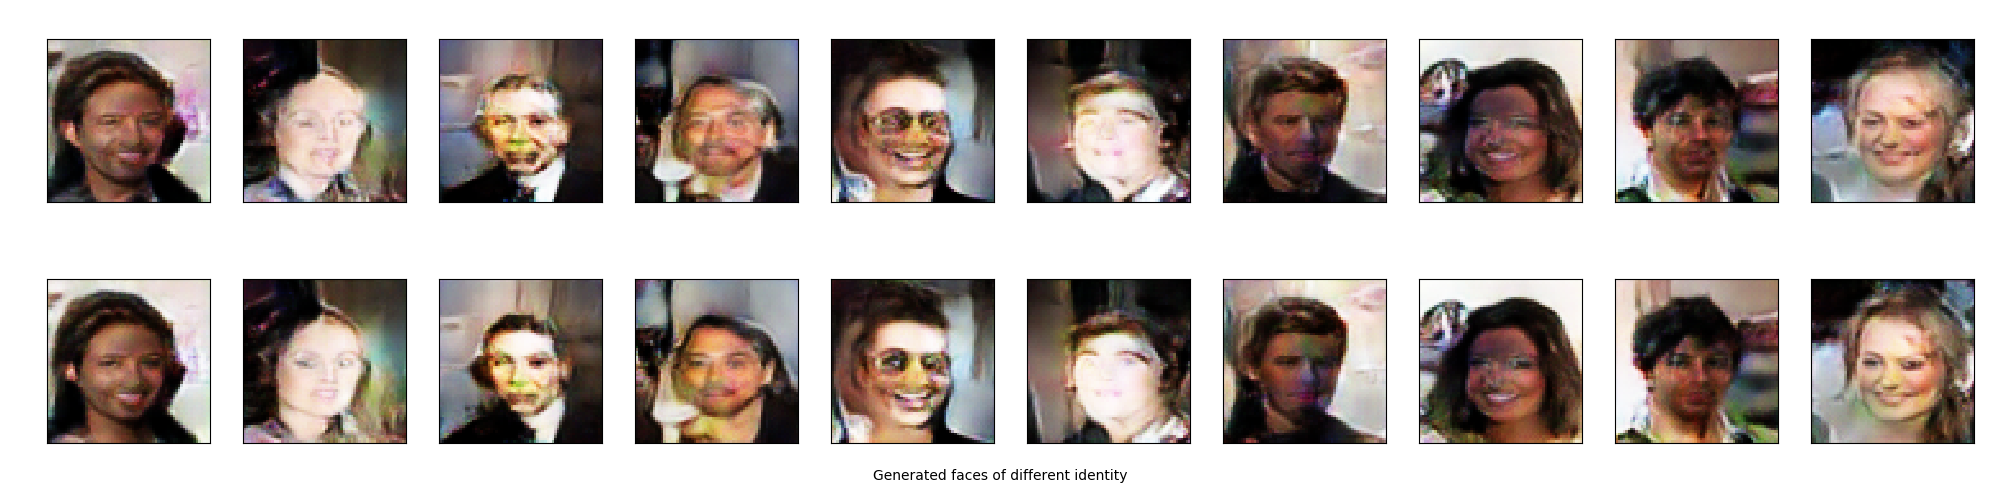
\includegraphics[width=5in]{image/identity_variation.png}
\end{center}
\caption{Generated faces under different epochs. The first row represents the result of young faces under different epochs. The second row represents the generated elder faces under different epochs.}
\label{figure: diff_identity}
\end{figure}
From Figure \ref{figure: diff_identity}, we can find several characteristics in our generated elder and young pairs. The first is that the eyes are drooping in elder faces whereas the eyes are big in young faces. Other characteristics we observed is that the skin for the elder is wrinkled and hairs are gray.
\subsection{Result of AE-cDCGAN}
In this section, we will show the result of AE-cDCGAN. Figure \ref{cdcgan_loss} shows the loss curve of AE-cDCGAN. The best-performed hyper parameter in this model determined was shown in Table \ref{table: AE-cDCGAN}.
\begin{figure}[H]
\begin{center}
  \centering
  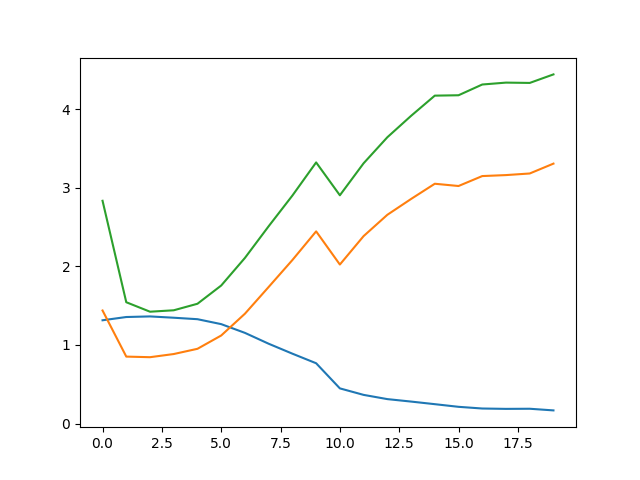
\includegraphics[scale=0.5]{image/loss_curve_AECDCGAN.png}
\end{center}
\caption{Loss change of AE-cDCGAN over 20 epochs. The orange line shows the loss of generator. The blue line shows the loss of discriminator. The green line shows the auto-encoder loss across the epoch.}
\label{cdcgan_loss}
\end{figure}

\begin{table}[H]
  \caption{Hyper Parameter of AE-cDCGAN}
  \label{table: AE-cDCGAN}
  \centering
  \begin{tabular}{cc}
    \toprule
    \cmidrule(r){1-2}
    Parameter    &Value\\
    \midrule
    Batch size           &128\\
    Alpha $\alpha$       &10\\
    Learning rate        &0.0001\\
    \bottomrule
  \end{tabular}
\end{table}
\subsubsection{Variation across difference significance of $\alpha$ for AE component}
In this part, we will explore the difference of parameter $\alpha$. Intuitively, when $\alpha$ grows up, the identity will be preserved more, which means the generated faces is more likely to be the same person of the original image. Through the experiment, it is noticeable that the generated faces are more alike with the original image when increasing value of $alpha$. However, when increasing the $alpha$, it is more difficult to make the model converge.
\begin{figure}[H]
\begin{center}
  \centering
  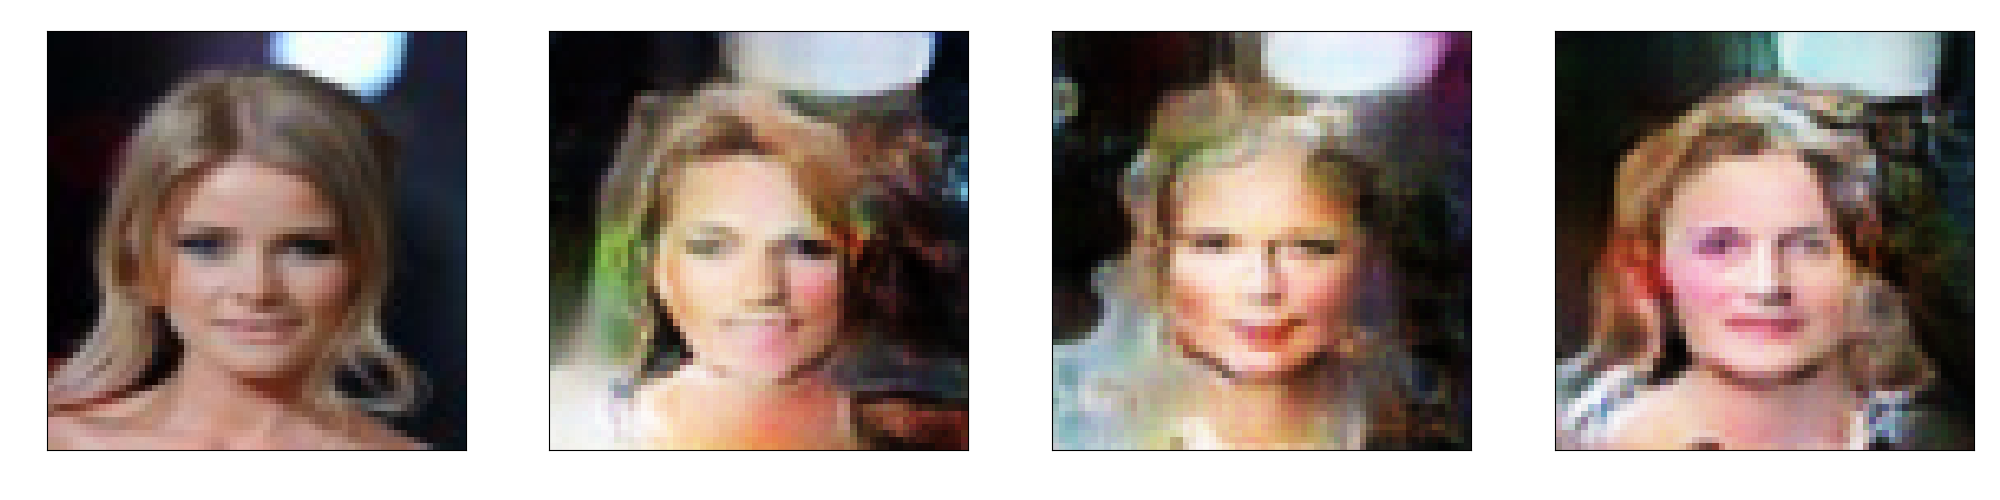
\includegraphics[scale=0.3]{image/diff_alpha.png}
\end{center}
\caption{Generated elder faces with different $alpha$ value. The left most image is the original image, and in the right side, they respectively represent $alpha=11,12,15$.}
\label{cdcgan_loss}
\end{figure}

\subsubsection{Aged Faces across different identities}
Figure \ref{aged_AEcDCGAN} shows the aged faces using AE-cDCGAN model. The first row are original faces and the second row are aged faces. Basing this model, it is evident that the identity has been preserved even though the background was not recovered. Besides, we can observe the difference between elder faces and the origin faces. For example, one of the most apparent characteristic is that the skin is wrinkled. Besides, the eyes look more drooped.
\begin{figure}[H]
\begin{center}
  \centering
  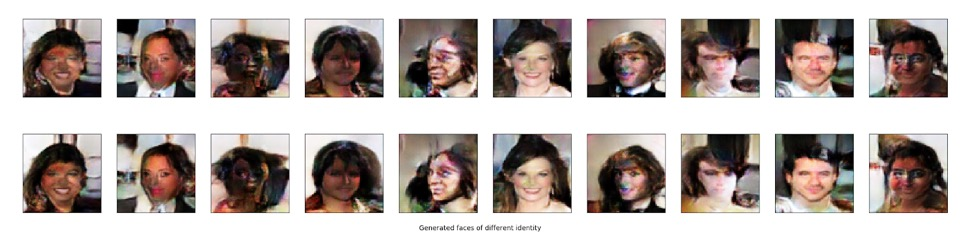
\includegraphics[width=5.5in]{image/identity.jpg}
\end{center}
\caption{Generated elder faces based on AE-cDCGAN. The first row is original faces. The second row is the aging faces.}
\label{aged_AEcDCGAN}
\end{figure}

\subsection{Result of StarGAN}

Figure \ref{stargan_loss} shows the loss of discriminator and generator. The StarGAN \cite{DBLP:journals/corr/abs-1711-09020} introduces an auxiliary classifier that helps a single discriminator to control multiple domains in that it decomposes the subjective into two term: one is the domain classification loss for fake images to optimize the generator and the other is the domain classification loss for real images to optimize the discriminator so that both the generator and discriminator are capable of convergence.

\begin{figure}[H]
\begin{center}
  \centering
  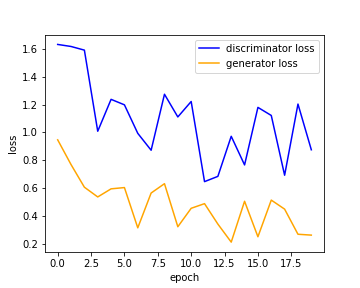
\includegraphics[width=3in]{image/stargan_loss.png}
\end{center}
\caption{Generated faces across different identities. The first row is the original input images, the second row is the elders generation of StarGAN.}
\label{stargan_loss}
\end{figure}

\subsubsection{Variation across the epoch}

Figure \ref{stargan_same_identity} shows the old faces under different epochs. The first image is the original input image. It is apparent that the elders images generated by StarGAN are much clearer than cDCGAN. Also the translation from youth to old is stable and natural compared to cDCGAN.

\begin{figure}[H]
\begin{center}
  \centering
  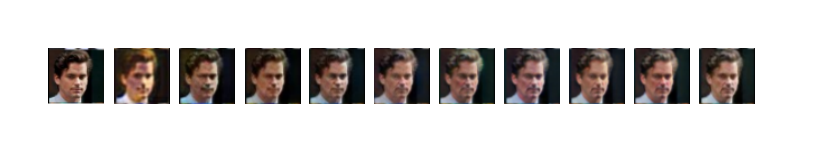
\includegraphics[width=6in]{image/stargan_same_identity.png}
\end{center}
\caption{Generated faces under different epochs. First image is the original input.}
\label{stargan_same_identity}
\end{figure}

\subsubsection{Generated faces across different identities}
Figure \ref{stargan_diff_identity} shows the generated faces across different input identities. It is obvious that all the old faces have the same characteristics of the elder, including wrinkles, eye morphogenesis and drooping cheek. It can also be seen from the figure that the hair color of the elder is slightly whiter than the young in some identities.

\begin{figure}[H]
\begin{center}
  \centering
  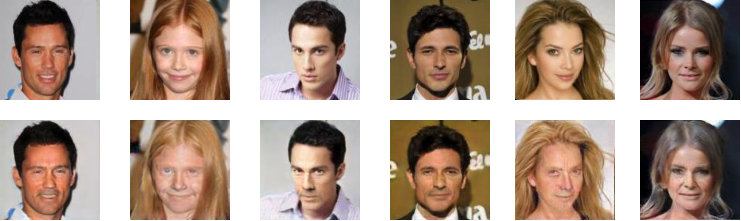
\includegraphics[width=5.5in]{image/stargan_diff_identity.png}
\end{center}
\caption{Generated faces across different identities. The first row is the original input images, the second row is the elders generation of StarGAN.}
\label{stargan_diff_identity}
\end{figure}

\subsection{Comparison}

Table \ref{comparison} shows the comparison of StarGAN and AE-cDCGAN on training time, number of images used for training and the quality of output. It takes roughly 37 minutes for StarGAN to train per epoch while AE-cDCGAN takes roughly 26 minutes to train per epoch. Because the imbalanced problem of the images with young/old attribute, we extract roughly $50,000$ young faces randomly to combine with the $50,000$ elder faces, similarly repeat 3 folds hence the AE-cDCGAN takes more resources for training. As for the quality for the generations, the aging faces generated by StarGAN are much clear, natural and realistic while aging faces generated by AE-cDCGAN are less clear and have oil-painting style.

\begin{table}[H]
\begin{center}
\setlength{\tabcolsep}{5mm}
\begin{tabular}{c|ccc}
\toprule
model & training time / epoch & \# images & quality \\
\midrule
StarGAN & $\sim 37$ mins & $202,599$ & realistic / clear \\
\midrule
AE-cDCGAN & $\sim 26$ mins & $275,190$ & oil-painting / less clear \\
\bottomrule
\end{tabular}
\caption{comparison between StarGAN and AE-cDCGAN on training time, number of images used for training and the quality of output.}
\label{comparison}
\end{center}
\end{table}

\section{Discussion and Conclusion}
AE-cDCGAN could achieve the goal of preserve the identity and compared with StarGAN, AE-cDCGAN is more lightweight and could complete the face aging process. However AE-cDCGAN generates less clear and oil-painting style faces because it is hard to converge since the auto encoder is not powerful enough to preserve the identity information as much as possible. In the future work, fine-tuning the model elaborately is an effective approach to improve the performance of AE-cDCGAN. We also want to amplify the signal of additional information so that the disparity of young and old attributes representation could be increased to help the convergence. Besides, cropping the image to remove background noise and only keep the face would also help improve the quality of the images generation.


\section{Contribution}
\paragraph{Guanghao Chen} Guanghao re implemented cDCGAN based on CelebA dataset. Furtherly, he proposed AE-cDCGAN model and implement it to complete face aging. Finally, he finished part of the report.

\paragraph{Qimin Chen} Qimin replicated the experiment of StarGAN and wrote the corresponding part of report. We discussed every details of the project together.

\paragraph{Yunfan Chen} Yunfan mainly focused on running the experiments and test the model. Yunfan also plotted the results needed for report and presentation.

\paragraph{Ke Xiao} Ke Xiao mainly focused on data pre-processing and made the powperpoint of presentation. We discussed every details of the project together.

\bibliography{citation}
\bibliographystyle{ieeetr}

\end{document}
